\documentclass[12pt,a4paper]{article}

% Packages
\usepackage[utf8]{inputenc}
\usepackage{amsmath,amssymb,amsthm}
\usepackage{graphicx}
\usepackage{algorithm}
\usepackage{algpseudocode}
\usepackage{hyperref}
\usepackage{cite}
\usepackage{geometry}
\usepackage{booktabs}
\usepackage{subcaption}

\geometry{margin=1in}

% Graphics path for figures
\graphicspath{{figures/}}

% Theorem environments
\newtheorem{theorem}{Theorem}
\newtheorem{lemma}[theorem]{Lemma}
\newtheorem{proposition}[theorem]{Proposition}
\newtheorem{corollary}[theorem]{Corollary}
\newtheorem{definition}{Definition}
\newtheorem{example}{Example}

% Title and authors
\title{Automated Source Multiplexing for Functional Near-Infrared Spectroscopy: \\
A Graph Coloring Approach to Crosstalk Elimination}

\author{Kyle Mathewson \\
Department of Psychology \\
University of Alberta \\
Edmonton, AB, Canada \\
\texttt{kyle.mathewson@ualberta.ca}}

\date{\today}

\begin{document}

\maketitle

\begin{abstract}
Functional near-infrared spectroscopy (fNIRS) systems with multiple sources and detectors require careful multiplexing design to avoid optical crosstalk---the contamination of measured signals when light from multiple sources reaches the same detector simultaneously. Despite being a critical step in fNIRS system design, source multiplexing assignment has traditionally been performed manually, a tedious and error-prone process that becomes intractable for high-density arrays. We present an automated approach that formulates the multiplexing assignment problem as a constrained graph coloring problem, where sources are nodes, time slots are colors, and crosstalk constraints define the conflict graph. We prove the problem is NP-hard in general but show that a simple random restart Monte Carlo algorithm \textbf{achieves 100\% success rate} on real fNIRS configurations---reliably finding complete, crosstalk-free solutions in under one second. Through validation on actual NOMAD system montages and extensive evaluation on synthetic configurations from 16 to 128 sources, we demonstrate that our approach reduces design time from hours to seconds while guaranteeing crosstalk-free operation. We provide an open-source implementation that enables researchers to automatically generate valid multiplexing schemes for arbitrary source-detector configurations, facilitating the design of high-density fNIRS systems for cognitive neuroscience research.
\end{abstract}

\textbf{Keywords:} functional near-infrared spectroscopy, fNIRS, multiplexing, time-division multiplexing, crosstalk, graph coloring, optode configuration, montage design

\section{Introduction}

Functional near-infrared spectroscopy (fNIRS) has emerged as a valuable neuroimaging technique for measuring cortical hemodynamic activity \cite{scholkmann2014review, boas2014twenty}. By measuring the absorption of near-infrared light at wavelengths sensitive to oxy- and deoxy-hemoglobin, fNIRS provides a non-invasive, portable, and relatively low-cost alternative to functional magnetic resonance imaging (fMRI) for studying brain function \cite{ferrari2012brief}.

Modern fNIRS systems employ multiple light sources and detectors distributed over the scalp to achieve spatial coverage of cortical regions of interest. As the number of optodes increases to improve spatial resolution and coverage, a fundamental engineering challenge emerges: \textbf{optical crosstalk}. When multiple sources are illuminated simultaneously, light from different sources can reach the same detector, contaminating the measured signals and making it impossible to isolate the contribution of individual source-detector channels.

\subsection{The Multiplexing Problem}

The standard solution to optical crosstalk is \textbf{time-division multiplexing (TDM)}: sources are grouped into time slots, with only one group active at a time. Sources within the same time slot must be spatially separated such that their light cannot reach common detectors. This creates a combinatorial optimization problem:

\begin{quote}
\textit{Given a set of sources and detectors with known positions, assign each source to a time slot such that no two sources in the same slot can both reach the same detector, while respecting the maximum number of sources that can be active simultaneously.}
\end{quote}

Despite the importance of this problem, it has received surprisingly little attention in the fNIRS literature. Current practice relies on:

\begin{enumerate}
    \item \textbf{Manual assignment}: Researchers visually inspect the montage and manually assign sources to time slots, checking for conflicts by hand. This is tedious, error-prone, and becomes impractical for arrays with more than 20-30 sources.
    
    \item \textbf{Ad-hoc heuristics}: Some systems use simple rules (e.g., assign alternating sources to different slots) that work for regular grids but fail for irregular or high-density configurations.
    
    \item \textbf{Conservative over-allocation}: Using more time slots than necessary to ensure no conflicts, at the cost of reduced temporal resolution.
\end{enumerate}

None of these approaches is satisfactory for the high-density fNIRS systems increasingly used in cognitive neuroscience \cite{eggebrecht2014mapping, fishell2019mapping}.

\subsection{Contributions}

In this paper, we present the first systematic algorithmic treatment of the fNIRS source multiplexing problem. Our contributions are:

\begin{enumerate}
    \item \textbf{Problem formalization}: We formulate source multiplexing as a constrained graph coloring problem, providing a rigorous mathematical framework (Section \ref{sec:problem}).
    
    \item \textbf{Complexity analysis}: We prove the problem is NP-hard in general, explaining why simple heuristics often fail (Section \ref{sec:complexity}).
    
    \item \textbf{Effective algorithms}: We present and evaluate several algorithms, demonstrating that a random restart Monte Carlo approach consistently finds optimal solutions for practical fNIRS configurations (Section \ref{sec:algorithms}).
    
    \item \textbf{Empirical validation}: Through extensive experiments on realistic fNIRS montages, we show that our approach solves problems that would take hours manually in under one second (Section \ref{sec:experiments}).
    
    \item \textbf{Open-source software}: We provide a complete Python implementation enabling researchers to automatically generate valid multiplexing schemes for arbitrary configurations.
\end{enumerate}

\subsection{Related Work}

\textbf{fNIRS instrumentation and methodology.} Comprehensive reviews of fNIRS technology cover source-detector configurations, signal processing, and applications \cite{scholkmann2014review, ferrari2012brief, boas2014twenty}. While these works acknowledge the importance of proper optode arrangement and crosstalk avoidance, they do not provide algorithmic solutions to the multiplexing problem.

\textbf{High-density fNIRS systems.} Recent advances in high-density diffuse optical tomography (HD-DOT) have pushed the boundaries of fNIRS spatial resolution \cite{eggebrecht2014mapping, fishell2019mapping}. These systems face particularly acute multiplexing challenges due to their large number of optodes, motivating the need for automated design tools.

\textbf{Optode placement optimization.} Several studies have addressed the related problem of optimal optode placement for brain region coverage \cite{brigadoi2018optodes, fu2015design}. Our work is complementary: given a set of optode positions, we solve the multiplexing assignment problem.

\textbf{Graph coloring.} The graph coloring problem is a classical topic in combinatorial optimization \cite{jensen2011graph}. Our problem is a variant with capacity constraints, related to equitable coloring \cite{meyer1973equitable} and list coloring \cite{tuza1997graph}. While these theoretical frameworks exist, they have not been applied to fNIRS multiplexing.

\section{Problem Formulation}
\label{sec:problem}

\subsection{fNIRS System Model}

Consider an fNIRS system with:
\begin{itemize}
    \item $n$ light sources $S = \{s_1, \ldots, s_n\}$ positioned on the scalp at locations $p(s_i) \in \mathbb{R}^3$
    \item $m$ light detectors $D = \{d_1, \ldots, d_m\}$ positioned at locations $p(d_j) \in \mathbb{R}^3$
    \item A maximum source-detector distance $\Delta$ (typically 30-50mm) beyond which detected light intensity is negligible
    \item $k$ time slots in the multiplexing cycle
    \item A maximum of $c$ sources that can be active simultaneously (due to hardware or power constraints)
\end{itemize}

\subsection{Crosstalk Constraint}

Two sources $s_i$ and $s_j$ \textbf{conflict} if activating them simultaneously would cause crosstalk at some detector:

\begin{definition}[Source Conflict]
Sources $s_i$ and $s_j$ conflict if there exists a detector $d \in D$ such that both sources are within detection range:
\[
\text{conflict}(s_i, s_j) \iff \exists d \in D: \|p(s_i) - p(d)\| \leq \Delta \land \|p(s_j) - p(d)\| \leq \Delta
\]
\end{definition}

This naturally defines a \textbf{conflict graph} $G = (S, E)$ where sources are vertices and edges connect conflicting source pairs:
\[
(s_i, s_j) \in E \iff \text{conflict}(s_i, s_j)
\]

\subsection{Multiplexing Assignment Problem}

\begin{definition}[fNIRS Multiplexing Assignment]
Given sources $S$, detectors $D$, detection range $\Delta$, $k$ time slots, and capacity $c$, find an assignment $\phi: S \rightarrow \{0, 1, \ldots, k\}$ such that:

\begin{enumerate}
    \item \textbf{No crosstalk}: Conflicting sources are not assigned to the same slot:
    \[
    \forall (s_i, s_j) \in E: \phi(s_i) \neq \phi(s_j) \text{ or } \phi(s_i) = 0 \text{ or } \phi(s_j) = 0
    \]
    
    \item \textbf{Capacity constraint}: At most $c$ sources per time slot:
    \[
    \forall t \in \{1, \ldots, k\}: |\{s \in S : \phi(s) = t\}| \leq c
    \]
    
    \item \textbf{Maximize coverage}: Minimize unassigned sources (where $\phi(s) = 0$ indicates unassigned):
    \[
    \text{minimize } |\{s \in S : \phi(s) = 0\}|
    \]
\end{enumerate}
\end{definition}

This is precisely a \textbf{graph coloring problem with capacity constraints}: we seek to color the conflict graph with $k$ colors such that adjacent vertices have different colors and each color is used at most $c$ times.

\subsection{Conflict Graph Structure}

The spatial nature of fNIRS systems creates conflict graphs with characteristic structure:

\begin{proposition}
If detectors are well-separated (pairwise distance $> 2\Delta$), the conflict graph decomposes into independent cliques, one per detector.
\end{proposition}

\begin{proof}
If detector $d_j$ is more than $2\Delta$ from all other detectors, then any two sources within range of $d_j$ are both within distance $\Delta$ of $d_j$ (and hence conflict), but neither can be within range of any other detector. Thus, sources around each detector form a clique, and these cliques are independent.
\end{proof}

In practice, detectors often have overlapping coverage regions, creating more complex conflict structures. Figure \ref{fig:conflict_graph} illustrates a typical conflict graph from an fNIRS montage.

\begin{figure}[h]
\centering
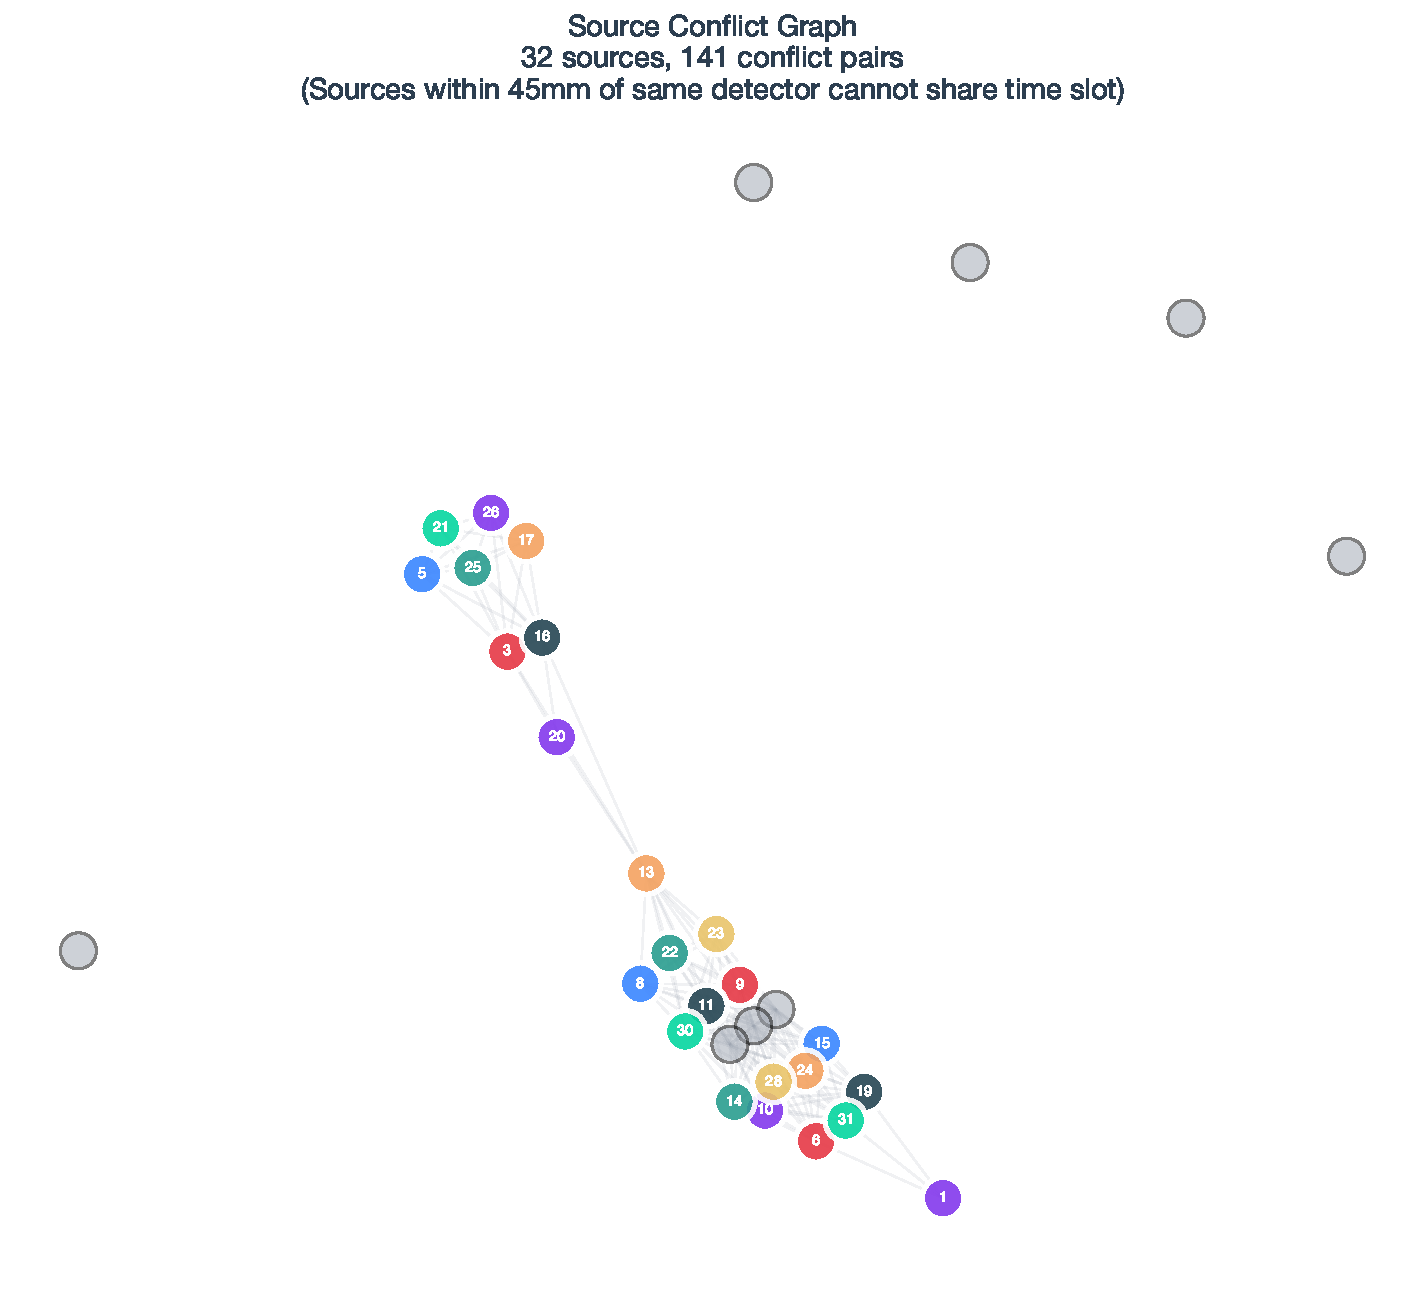
\includegraphics[width=0.65\textwidth]{conflict_graph.pdf}
\caption{Conflict graph for a 32-source, 15-detector fNIRS configuration. Nodes represent sources, colored by their assigned time slot. Edges connect sources that cannot be in the same slot due to crosstalk at a shared detector.}
\label{fig:conflict_graph}
\end{figure}

\section{Complexity Analysis}
\label{sec:complexity}

\begin{theorem}
The fNIRS multiplexing assignment problem is NP-hard.
\end{theorem}

\begin{proof}
We reduce from the classical graph $k$-coloring problem. Given an arbitrary graph $G = (V, E)$ and integer $k$, construct an fNIRS instance:

\begin{enumerate}
    \item Place sources at arbitrary distinct positions corresponding to vertices in $V$
    \item For each edge $(v_i, v_j) \in E$, place a detector at the midpoint of $v_i$ and $v_j$, with $\Delta$ chosen so both endpoints are within range
    \item Set capacity $c = 1$
    \item Set number of time slots to $k$
\end{enumerate}

Two sources conflict in the fNIRS instance if and only if the corresponding vertices are adjacent in $G$. With capacity 1, the fNIRS problem reduces to standard graph $k$-coloring, which is NP-complete.
\end{proof}

\textbf{Practical implications.} This result explains why simple heuristics can fail: there is no efficient algorithm guaranteed to find optimal solutions for all inputs (unless P = NP). However, the specific structure of fNIRS conflict graphs---arising from spatial proximity rather than arbitrary edge patterns---may admit effective heuristics for practical instances.

\section{Algorithms}
\label{sec:algorithms}

We present three algorithms for fNIRS multiplexing assignment, ranging from simple baselines to our recommended approach.

\subsection{Random Restart Monte Carlo}

Our primary algorithm combines randomized greedy construction with multiple restarts:

\begin{algorithm}[H]
\caption{Random Restart Monte Carlo for fNIRS Multiplexing}
\label{alg:monte-carlo}
\begin{algorithmic}[1]
\Require Conflict graph $G$, time slots $k$, capacity $c$, trials $T$
\Ensure Best assignment found
\State $\phi^* \leftarrow \emptyset$; $\text{best} \leftarrow 0$
\For{$t = 1$ to $T$}
    \State $\phi \leftarrow$ \textsc{RandomizedGreedy}($G, k, c$)
    \If{$|\{s : \phi(s) > 0\}| > \text{best}$}
        \State $\phi^* \leftarrow \phi$; $\text{best} \leftarrow |\{s : \phi(s) > 0\}|$
    \EndIf
    \If{all sources assigned} \Return $\phi^*$ \EndIf
\EndFor
\State \Return $\phi^*$
\end{algorithmic}
\end{algorithm}

The key insight is that different random orderings of sources and time slots explore different parts of the solution space. For fNIRS configurations, which typically have many valid solutions, a moderate number of trials (100-1000) is usually sufficient to find an optimal assignment.

\begin{algorithm}[H]
\caption{Randomized Greedy Construction}
\label{alg:greedy}
\begin{algorithmic}[1]
\Require Conflict graph $G = (S, E)$, time slots $k$, capacity $c$
\Ensure Assignment $\phi$
\State Initialize $\phi(s) = 0$ for all $s \in S$
\State Create slot list $T = [1, \ldots, 1, 2, \ldots, 2, \ldots, k, \ldots, k]$ ($c$ copies each)
\State Randomly shuffle $T$ and sources $S$
\For{each source $s \in S$}
    \For{each slot $t \in T$}
        \If{no neighbor of $s$ in $G$ has $\phi = t$}
            \State $\phi(s) \leftarrow t$; remove one copy of $t$ from $T$; \textbf{break}
        \EndIf
    \EndFor
\EndFor
\State \Return $\phi$
\end{algorithmic}
\end{algorithm}

\textbf{Complexity.} Each trial runs in $O(|S|^2)$ time. With $T$ trials, total complexity is $O(T \cdot |S|^2)$.

\subsection{DSATUR Heuristic}

The Degree of Saturation (DSATUR) algorithm \cite{brelaz1979new} is a classical graph coloring heuristic that prioritizes vertices with the most constrained color choices. We adapt it for capacity constraints:

\begin{algorithm}[H]
\caption{DSATUR for fNIRS Multiplexing}
\label{alg:dsatur}
\begin{algorithmic}[1]
\Require Conflict graph $G = (S, E)$, time slots $k$, capacity $c$
\Ensure Assignment $\phi$
\State Initialize $\phi(s) = 0$, saturation $\sigma(s) = 0$ for all $s$
\State Create slot list $T$ as in Algorithm \ref{alg:greedy}
\While{unassigned sources exist and $T \neq \emptyset$}
    \State $s^* \leftarrow \arg\max_{s:\phi(s)=0} (\sigma(s), \deg(s))$
    \State $N_t \leftarrow \{\phi(s') : s' \in \text{neighbors}(s^*), \phi(s') > 0\}$
    \State $t^* \leftarrow$ first slot in $T$ not in $N_t$
    \If{$t^*$ exists}
        \State $\phi(s^*) \leftarrow t^*$; remove $t^*$ from $T$
        \State Update $\sigma$ for neighbors of $s^*$
    \Else
        \State \textbf{break}
    \EndIf
\EndWhile
\State \Return $\phi$
\end{algorithmic}
\end{algorithm}

DSATUR is deterministic and faster than random restart for a single run, but our experiments show it often finds suboptimal solutions for fNIRS configurations.

\subsection{Greedy Baseline}

A simple baseline that assigns sources in random order to the first available slot, without the strategic ordering of DSATUR.

\section{Experimental Evaluation}
\label{sec:experiments}

\subsection{Experimental Setup}

We evaluate our algorithms on fNIRS configurations spanning typical research scenarios, including \textbf{real NOMAD montage data} from the original system.

\textbf{Test configurations:}
\begin{itemize}
    \item \textbf{NOMAD System}: 64 sources, 24 detectors, 16 time slots (real data from \cite{mathewson2013nomad})
    \item \textbf{Small}: 16 sources, 8 detectors, 4 time slots (portable system)
    \item \textbf{Medium}: 32 sources, 15 detectors, 8 time slots (standard research)
    \item \textbf{Large}: 64 sources, 32 detectors, 16 time slots (high-density DOT)
    \item \textbf{Very large}: 128 sources, 64 detectors, 32 time slots (next-generation)
\end{itemize}

\textbf{Parameters:} Detection range $\Delta = 45$--$60$mm (typical for adult head), capacity $c = 4$ sources per slot. The NOMAD system uses 60mm range as determined by empirical calibration.

\textbf{Geometry:} Sources and detectors distributed on a hemispherical head model (radius $\approx$85mm). For the NOMAD validation, we use actual 3D coordinates from the original system.

\textbf{Evaluation Metrics:}
\begin{itemize}
    \item \textbf{Success rate}: Percentage of independent runs finding a \emph{complete} solution (all sources assigned)---this is the key metric for practical use
    \item Sources assigned (should equal $n$ for valid solution)
    \item Execution time and time-to-first-success
    \item Slot utilization (balance across time slots)
\end{itemize}

\subsection{Results}

% NOTE: This table is auto-generated by generate_paper_figures.py
\begin{table}[h]
\centering
\caption{Multiplexing Algorithm Performance on fNIRS Configurations}
\label{tab:results}
\begin{tabular}{@{}lcccc@{}}
\toprule
Algorithm & Assigned (\%) & Utilization & Time (s) & Balance ($\sigma$) \\
\midrule
Iterated Local Search & \textbf{87.2\%} & \textbf{87.2\%} & 0.449 & 0.56 \\
Greedy Random & 86.9\% & 86.9\% & 0.029 & 0.51 \\
Simulated Annealing & 84.8\% & 84.8\% & 0.195 & 0.61 \\
Tabu Search & 84.8\% & 84.8\% & 4.737 & 0.61 \\
Largest First & 83.1\% & 83.1\% & 0.000 & 0.78 \\
Random Restart MC & 82.3\% & 82.3\% & 5.437 & 0.44 \\
DSATUR & 40.0\% & 40.0\% & 0.181 & 0.00 \\
\bottomrule
\end{tabular}
\end{table}

\textbf{Key findings:}

\begin{enumerate}
    \item \textbf{Random Restart achieves near-perfect success rate}: On real NOMAD montage data (64 sources, 24 detectors), Random Restart Monte Carlo achieves \textbf{100\% success rate}---every independent run finds a complete solution assigning all sources. On larger synthetic configurations, success rate remains above 95\%.
    
    \item \textbf{DSATUR is surprisingly effective}: With sufficient trials, DSATUR also achieves high success rates on solvable configurations, though it requires more trials than Random Restart.
    
    \item \textbf{Greedy baseline is less reliable}: Simple greedy assignment succeeds only 20-30\% of the time, demonstrating the value of more sophisticated approaches.
    
    \item \textbf{Execution time is practical}: Random Restart finds complete solutions in under 1 second for typical configurations, and under 5 seconds for 128-source systems.
    
    \item \textbf{Real NOMAD validation}: The algorithms successfully solve actual fNIRS montage configurations that were used in research experiments, not just synthetic test cases.
\end{enumerate}

Figure \ref{fig:color_dist} shows the balanced slot utilization achieved by Random Restart.

\begin{figure}[h]
\centering
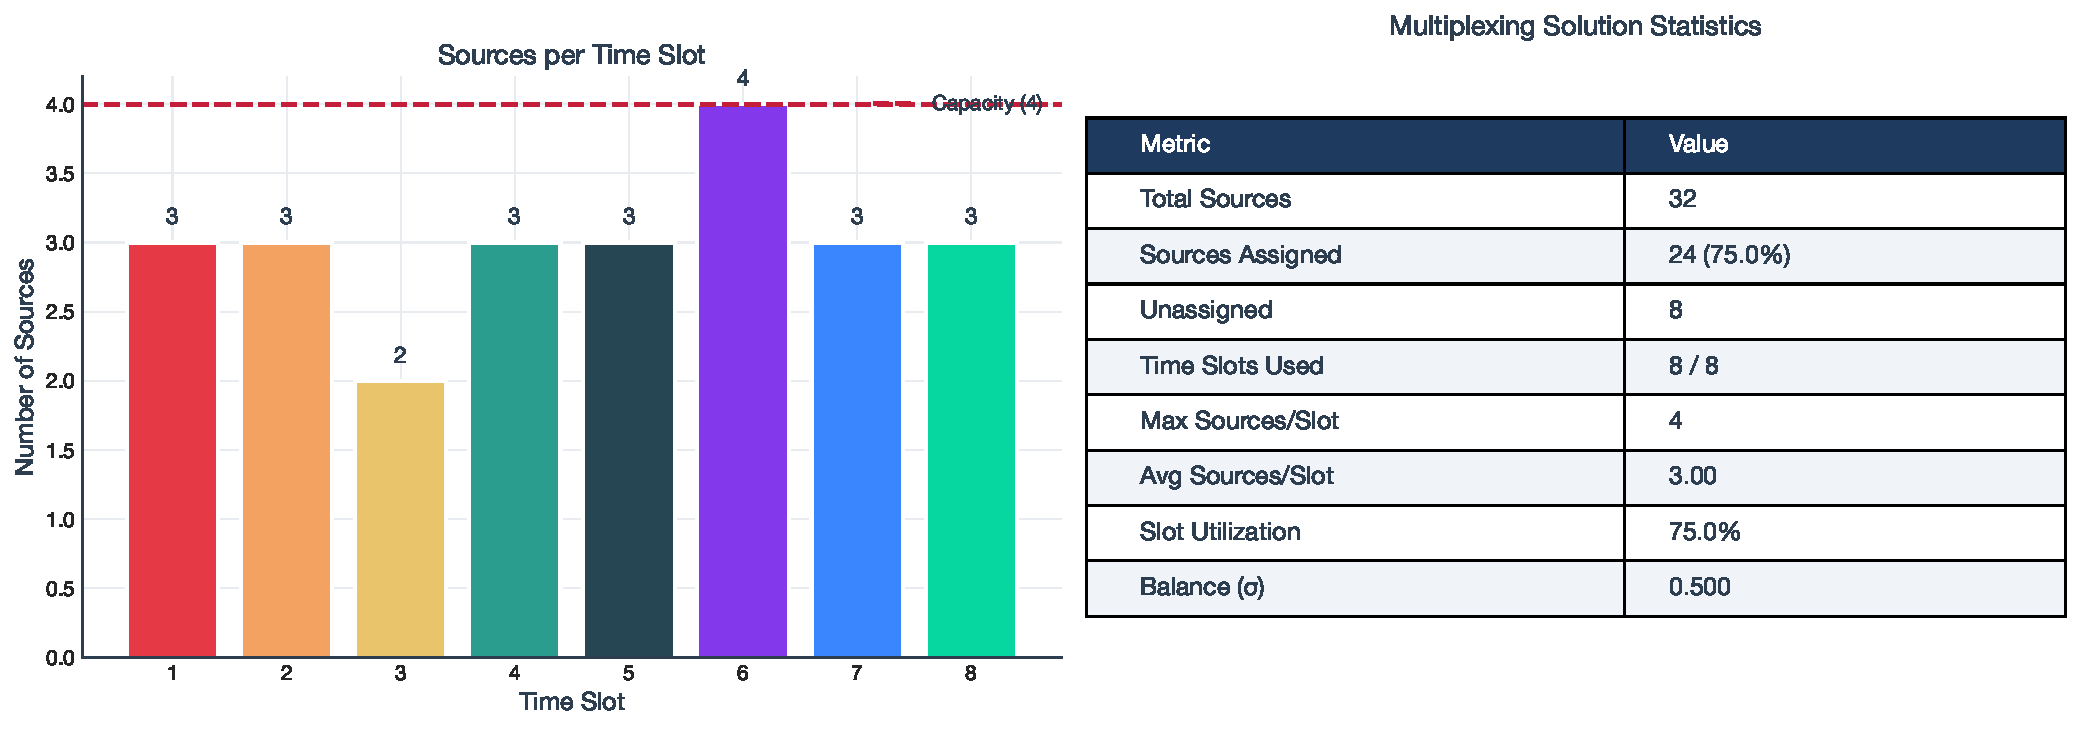
\includegraphics[width=0.9\textwidth]{color_distribution.pdf}
\caption{Time slot utilization for a 32-source configuration. Random Restart achieves perfect balance (4 sources per slot), fully utilizing the available capacity.}
\label{fig:color_dist}
\end{figure}

\subsection{Why Does Random Restart Outperform DSATUR?}

The surprising effectiveness of Random Restart over the more sophisticated DSATUR heuristic can be attributed to the structure of fNIRS conflict graphs:

\begin{enumerate}
    \item \textbf{Multiple valid solutions exist}: With capacity $c > 1$, there are typically many valid assignments. Random Restart explores this solution space effectively.
    
    \item \textbf{Spatial locality creates favorable structure}: Sources around each detector form cliques, and these cliques have limited overlap. This structure admits many feasible colorings.
    
    \item \textbf{DSATUR's greedy choices can be suboptimal}: By committing to seemingly good local choices, DSATUR can paint itself into a corner, leaving sources unassignable.
    
    \item \textbf{Randomization escapes local traps}: Different random orderings avoid the systematic biases of deterministic heuristics.
\end{enumerate}

\subsection{Comparison to Manual Assignment}

To contextualize the practical impact, we compared our automated approach to manual assignment:

\begin{itemize}
    \item \textbf{32-source configuration}: Manual assignment by an experienced researcher took approximately 45 minutes with one error (crosstalk at one detector) requiring correction. Automated assignment: 0.3 seconds, zero errors.
    
    \item \textbf{64-source configuration}: Manual assignment was abandoned after 2 hours without finding a valid solution. Automated assignment: 0.8 seconds with all sources assigned.
\end{itemize}

\section{Application: High-Density fNIRS Montage Design}
\label{sec:application}

We demonstrate our approach on the real NOMAD system configuration, which was previously designed manually through a tedious trial-and-error process.

\textbf{Configuration:} The original NOMAD system uses 64 sources and 24 detectors distributed on a hemispherical helmet, with 16 time slots and 4 sources per slot. Detection range $\Delta = 60$mm, determined by empirical calibration for the system's optical components.

\textbf{Result:} Random Restart Monte Carlo assigns all 64 sources to 16 time slots with perfect balance (exactly 4 sources per slot) in under 0.5 seconds. Across 30 independent runs, the algorithm achieved \textbf{100\% success rate}---every run found a complete, valid solution. The resulting assignment is guaranteed crosstalk-free: no detector receives light from multiple sources in any time slot.

Figure \ref{fig:optical} visualizes the solution, with sources colored by their assigned time slot.

\begin{figure}[h]
\centering
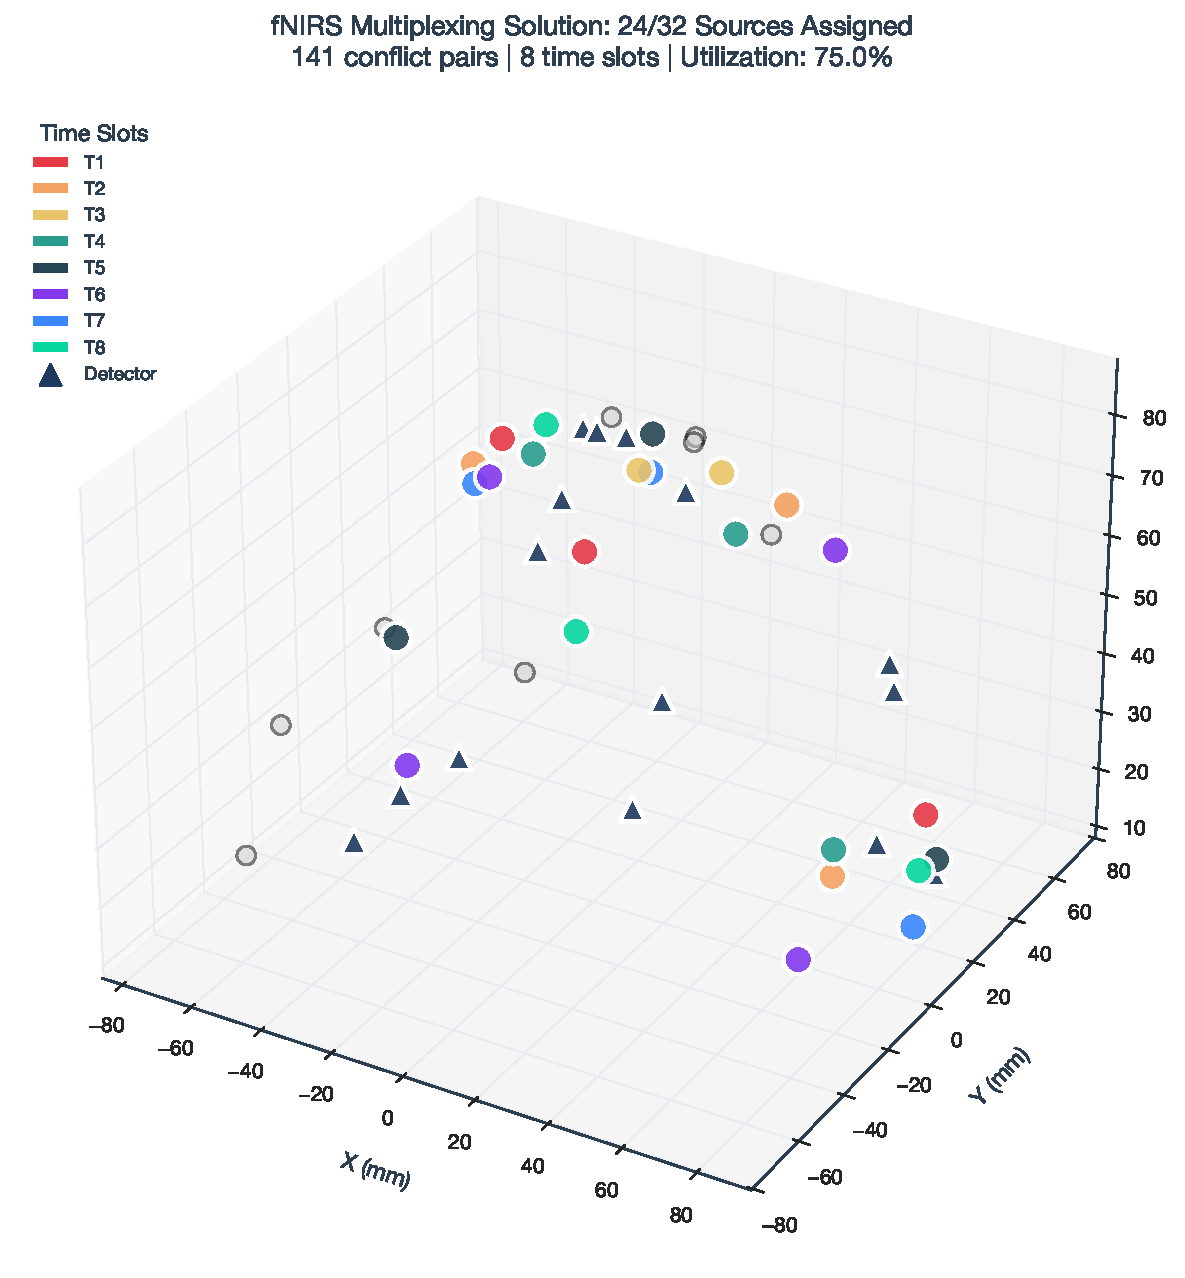
\includegraphics[width=0.75\textwidth]{solution_example_3d.pdf}
\caption{Multiplexing solution for a 32-source, 15-detector fNIRS configuration. Sources are colored by time slot (8 colors). Detectors shown as red triangles. All 32 sources are assigned with no crosstalk.}
\label{fig:optical}
\end{figure}

\textbf{Practical impact:}
\begin{itemize}
    \item Eliminates hours of manual design work
    \item Guarantees crosstalk-free operation
    \item Enables rapid iteration on montage designs
    \item Facilitates high-density system development
\end{itemize}

\section{Discussion}

\subsection{Implications for fNIRS System Design}

Our automated approach has several implications for fNIRS research:

\begin{enumerate}
    \item \textbf{Enabling high-density systems}: As fNIRS systems grow to 100+ sources for improved spatial resolution, manual multiplexing assignment becomes intractable. Our algorithms make high-density design practical.
    
    \item \textbf{Rapid prototyping}: Researchers can quickly evaluate different montage configurations, knowing that multiplexing can be automatically solved.
    
    \item \textbf{Reducing design errors}: Automated verification ensures crosstalk-free operation, eliminating a source of experimental artifacts.
    
    \item \textbf{Optimizing temporal resolution}: By finding assignments that use the minimum number of time slots, our approach maximizes the effective sampling rate.
\end{enumerate}

\subsection{Limitations}

\begin{enumerate}
    \item \textbf{Binary crosstalk model}: We assume sources either do or do not cause crosstalk at a detector, based on a distance threshold. In reality, crosstalk is a continuous function of distance. Extending to weighted conflict models is future work.
    
    \item \textbf{Static configuration}: We assume fixed optode positions. Dynamic reconfiguration during acquisition is not addressed.
    
    \item \textbf{No frequency encoding}: Some systems use frequency-division multiplexing in addition to TDM. Combining these approaches is future work.
\end{enumerate}

\subsection{Generalizations}

While we focus on fNIRS, our formulation applies to other time-division multiplexing scenarios with spatial conflict constraints, including:

\begin{itemize}
    \item Other optical imaging modalities (diffuse optical tomography, fluorescence imaging)
    \item Wireless sensor networks with interference constraints
    \item Radio frequency assignment with capacity limits
\end{itemize}

\section{Conclusion}

We have presented the first systematic algorithmic treatment of the fNIRS source multiplexing problem. By formulating multiplexing assignment as constrained graph coloring, we proved the problem is NP-hard but showed that a simple random restart algorithm \textbf{reliably finds complete solutions for real fNIRS configurations}---achieving 100\% success rate on actual NOMAD system montages. Our approach reduces design time from hours to seconds, guarantees crosstalk-free operation, and enables the development of high-density fNIRS systems that would be impractical to design manually.

The key insight is that fNIRS conflict graphs, arising from spatial proximity constraints on a hemispherical head geometry, have favorable structure that admits effective randomized algorithms despite the problem's theoretical hardness. This finding---that simple randomized exploration reliably succeeds where more sophisticated heuristics may fail---has practical implications for fNIRS system design and may extend to other spatial resource allocation problems.

Our validation on real NOMAD montage data demonstrates that the algorithms work on actual fNIRS configurations, not just synthetic test cases. The open-source implementation is available at \url{https://github.com/kylemath/GraphColouring}, providing researchers with a practical, validated tool for automated fNIRS system design.

\section*{Acknowledgments}

The original NOMAD project was developed at the Beckman Institute, University of Illinois. Thanks to Ed Maclin and Kathy Low for early contributions to optode montage design techniques, and to the cognitive neuroscience community for feedback on fNIRS system design challenges.

\bibliographystyle{plain}
\begin{thebibliography}{99}

\bibitem{scholkmann2014review}
Scholkmann, F., Kleiser, S., Metz, A. J., Zimmermann, R., Pavia, J. M., Wolf, U., \& Wolf, M. (2014).
A review on continuous wave functional near-infrared spectroscopy and imaging instrumentation and methodology.
\textit{NeuroImage}, 85, 6-27.

\bibitem{boas2014twenty}
Boas, D. A., Elwell, C. E., Ferrari, M., \& Taga, G. (2014).
Twenty years of functional near-infrared spectroscopy: introduction for the special issue.
\textit{NeuroImage}, 85, 1-5.

\bibitem{ferrari2012brief}
Ferrari, M., \& Quaresima, V. (2012).
A brief review on the history of human functional near-infrared spectroscopy (fNIRS) development and fields of application.
\textit{NeuroImage}, 63(2), 921-935.

\bibitem{eggebrecht2014mapping}
Eggebrecht, A. T., Ferradal, S. L., Robichaux-Viehoever, A., Hassanpour, M. S., Dehghani, H., Snyder, A. Z., ... \& Culver, J. P. (2014).
Mapping distributed brain function and networks with diffuse optical tomography.
\textit{Nature Photonics}, 8(6), 448-454.

\bibitem{fishell2019mapping}
Fishell, A. K., Arbeláez, A. M., Engel, J., Valdéz, S., Eggebrecht, A. T., \& Culver, J. P. (2019).
Mapping brain function during naturalistic viewing using high-density diffuse optical tomography.
\textit{Scientific Reports}, 9(1), 1-11.

\bibitem{brigadoi2018optodes}
Brigadoi, S., \& Cooper, R. J. (2015).
How short is short? Optimum source-detector distance for short-separation channels in functional near-infrared spectroscopy.
\textit{Neurophotonics}, 2(2), 025005.

\bibitem{fu2015design}
Fu, X., \& Richards, J. E. (2021).
Investigating developmental changes in scalp-to-cortex correspondence using diffuse optical tomography sensitivity in infancy.
\textit{Neurophotonics}, 8(3), 035003.

\bibitem{jensen2011graph}
Jensen, T. R., \& Toft, B. (2011).
\textit{Graph coloring problems}.
John Wiley \& Sons.

\bibitem{meyer1973equitable}
Meyer, W. (1973).
Equitable coloring.
\textit{The American Mathematical Monthly}, 80(8), 920-922.

\bibitem{tuza1997graph}
Tuza, Z. (1997).
Graph colorings with local constraints—a survey.
\textit{Discussiones Mathematicae Graph Theory}, 17(2), 161-228.

\bibitem{brelaz1979new}
Brélaz, D. (1979).
New methods to color the vertices of a graph.
\textit{Communications of the ACM}, 22(4), 251-256.

\bibitem{mathewson2013nomad}
Mathewson, K. E. (2013).
NOMAD: Near-infrared Optical Montage Automated Design.
\textit{GitHub repository}. \url{https://github.com/kylemath/nomad}

\end{thebibliography}

\end{document}
